\section{Environment plug-in}

\subsection{Overview}

The architecture of the plug-in comes from
\cite{DeclarativeArchitecture}, to provide an intuitive way of
building an environment: by drawing features on a map. The most
difficult part in this approach is that intersecting features are
allowed and should give a result consistent with user expectations.

As a starting point, we focused on generating a height map, using the
concepts from \cite{FeatureTree}. It had the advantage of being able
to merge features smoothly whenever they intersect, rather than using
the more convoluted conflict-resolution mechanism of
\cite{DeclarativeArchitecture}.

\bigskip

The basic unit managed by this plugin is a \emph{feature}, which lies
in a certain area, has a certain height profile and knows how to
interact with the other features that may intersect it. From the
collection of all the features drawn on the map by the user, our
plug-in builds a tree encoding how to build the final height map by
successively merging sets of features together.  %TODO: mention models
(e.g. trees for forests)


%% Mettre un example de carte + rendu ici ?

\subsection{Features}

\subsubsection{Mountains}

Our first implementation of the Mountain feature corresponded to what
is presented in \cite{FeatureTree}, where mountains are generated
procedurally. However, the 2D random functions we tried did not yield
satisfying results. That's why we switched to another version, where
we import at random a part of a heightmap taken from a website
\cite{terrain-party}. This website import the heightmaps through
satellite imaging.

\subsubsection{Cities}

We planned a feature that could generate cities, following a
three-step process. First, draw the street network. For this task we
chose to use the method of \cite{StreetTensors}, which provides a more
or less intuitive way for the user to control the output. Then, divide
each street-delimited block into parcels. We chose to follow the
approach of \cite{PGParcels}, which seemed to give realistic
results. Finally, put a building in each parcel. We did not look much
into that last part because using buildings of random height was
thought to be a reasonable approximation.

However, even the first step turned out to be challenging to
implement. The principle of the chosen method was to describe the
shape of the street network by a tensor field, mapping points to $2
\times 2$ matrices. It is described by a combination of basic fields
given by the user. The streets are then drawn as the stream lines of
the eigenvectors of the field. The main issue here was to represent
the street network under construction so that:
\begin{itemize}
  \item street drawing starts from points belonging to old streets and
satisfying certain constraints
  \item new intersections are correctly handled while drawing a street
  \item the right eigenvector is always chosen
\end{itemize} without having to reimplement the computation of
eigenvectors or the numerical approximation of a differential
equation.

%% On ne parle pas trop de ce qui allait pas là non ?

\subsection{Graphical User Interface (GUI)}

A picture of the interface is presented in
Fig.~\ref{fig:env-gui1}. Using the interface, the user can choose the
feature he wants to draw. He can then draw it using a pencil
integrated in Blender, drawing polygons here. After having completed
the drawing of the features, the user can ask for the generation of
the environment. It can then hide the polygons, and also modify
parameters that are feature-specific.

\begin{figure}
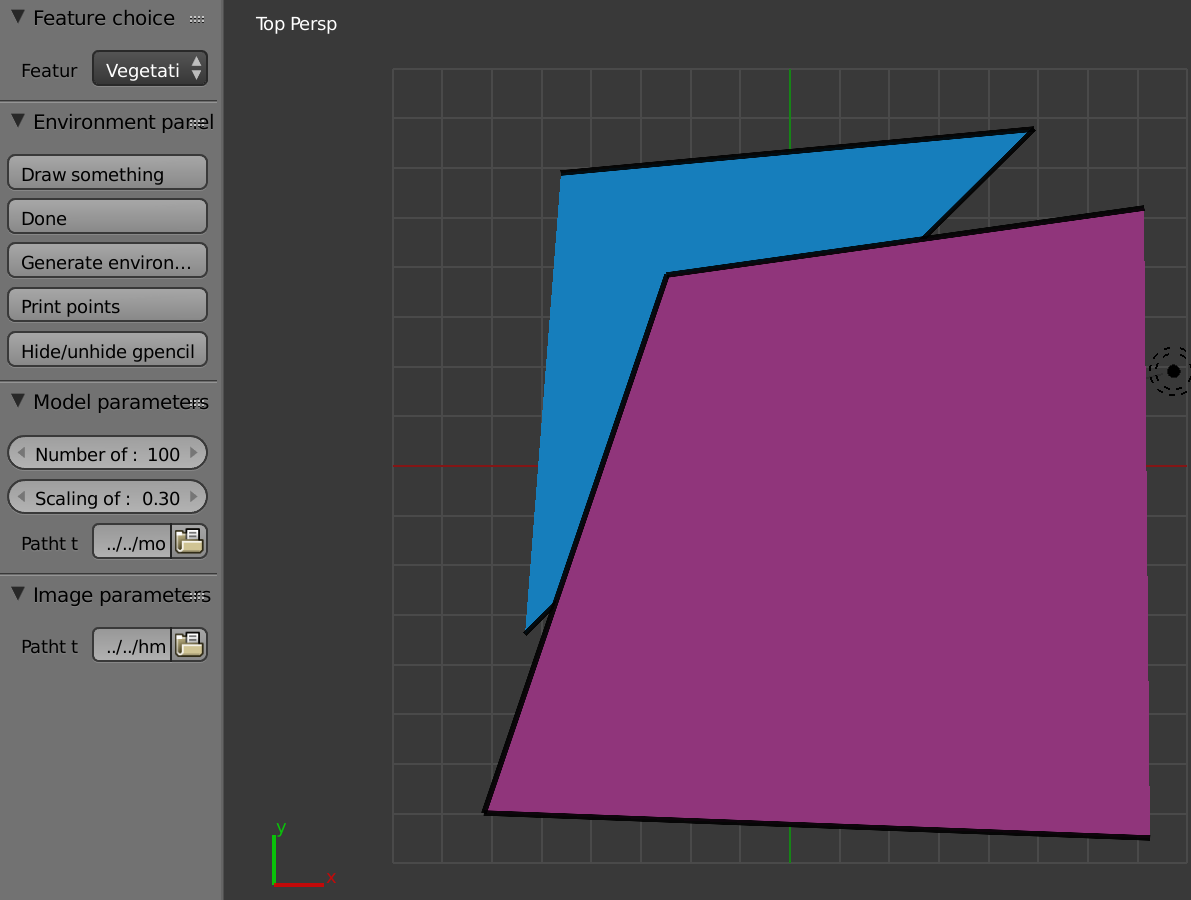
\includegraphics[width=\textwidth]{img/env_gui1.png}
\caption{GUI of the Environment plug-in, with two features (in blue
and magenta)}
\label{fig:env-gui1}
\end{figure}

%% Eventuellement : faire deux images, une du dessin des features, et
%% une de la génération ?
